\part{The main loop}
\frame{\partpage}

\begin{frame}{Basic game architecture}
    \begin{itemize}
        \pause\item CPUs execute \textbf{sequences of instructions} 
            \begin{itemize}
                \pause\item At the CPU level, there is no such thing as ``when $X$ happens, do $Y$'' 
                \pause\item Instead: ``keep checking whether $X$ has happened; if so, do $Y$'' 
            \end{itemize}
        \pause\item Thus games need to have a \textbf{main loop} 
        \pause\item The main loop is usually part of the game's \textbf{engine} 
            \begin{itemize}
                \pause\item E.g. Unreal implements the main loop for you 
                \pause\item E.g. PyGame isn't a game engine, so you have to implement your own main loop
            \end{itemize}
    \end{itemize}
\end{frame}

\begin{frame}{The basic main loop}
    \pause The most basic main game loop does \textbf{two} things: 
    \begin{enumerate}
        \pause\item \textbf{Update} the state of the game 
            \begin{itemize}
            	\pause\item Handle player input
                \pause\item Update physics, collision detection, AI etc. 
                \pause\item Do any game-specific updates 
            \end{itemize}
        \pause\item \textbf{Render} the game to the screen
            \begin{itemize}
            	\pause\item Game world 
                \pause\item User interface
            \end{itemize}
    \end{enumerate}
    \pause It does these \textbf{once per frame} (typically 30 or 60 times per second)
\end{frame}

\begin{frame}[fragile]{The basic main loop}
    \begin{lstlisting}
bool running = true;

while (running)
{
    update();
    render();
}
    \end{lstlisting}
\end{frame}

\begin{frame}{Rendering}
    \begin{itemize}
        \pause\item This is where you draw the \textbf{current state of the game} to the screen 
        \pause\item Also draw any \textbf{heads-up display (HUD)} elements,
            e.g.\ score, lives, mini-map, etc. 
        \pause\item Most modern game engines \textbf{clear the screen and redraw everything} on every frame 
    \end{itemize}
\end{frame}

\begin{frame}{Screen refresh rate}
    \begin{itemize}
        \pause\item Old CRT monitors worked by scanning an electron beam down the screen
            \begin{itemize}
                \pause\item \url{https://www.youtube.com/watch?v=lRidfW_l4vs} 
            \end{itemize}
        \pause\item Hence the term \textbf{(vertical) refresh rate} 
        \pause\item Refresh rate is measured in \textbf{cycles per second} i.e.\ \textbf{Hz} 
        \pause\item Other monitor technologies work differently, but still refresh the screen at regular intervals
    \end{itemize}
\end{frame}

\begin{frame}{Frame rate}
    \begin{itemize}
        \pause\item We generally want to sync it up so that \newline
            \textbf{one display refresh = one main loop iteration} 
        \pause\item If the main loop runs too slowly, we get ``lag'' 
        \pause\item If the main loop runs too quickly, we waste resources on drawing things faster than the display can show them
    \end{itemize}
\end{frame}

\begin{frame}{Limiting the frame rate}
    \begin{itemize}
        \pause\item The game's main loop is generally synchronised to the screen refresh rate 
        \pause\item However, refresh rates can vary
            \begin{itemize}
                \pause\item Older TVs: $\sim$ 30Hz
                \pause\item HDTVs and standard monitors: 60Hz
                \pause\item VR headsets: 90Hz
                \pause\item High-end gaming monitors: 120Hz or higher
            \end{itemize}
    \end{itemize}
\end{frame}

\begin{frame}{Limiting the update rate}
    \begin{itemize}
        \pause\item Having the update frequency depend on the refresh rate would be bad!
            \begin{itemize}
                \pause\item The game could appear to run in slow or fast motion,
                    completely changing the gameplay 
            \end{itemize}
        \pause\item This was the situation on older consoles:
            American/Japanese versions of games actually ran a little faster
            than European versions,
            due to the NTSC TV standard having a higher refresh rate than PAL!
    \end{itemize}
\end{frame}

\begin{frame}[fragile]{Variable time step}
    \begin{itemize}
        \pause\item Have the update step depend on the \textbf{elapsed time since the last update} 
        \pause\item Also known as the \textbf{delta time} 
        \pause\item E.g.\ if the game is running at a steady 60FPS, delta time $= \frac{1}{60}$
        \pause\item So instead of this:
    \end{itemize}
    \begin{lstlisting}
player.positionX += player.velocityX;
    \end{lstlisting}
    \begin{itemize}
        \pause\item do this:
    \end{itemize}
    \begin{lstlisting}
player.positionX += player.velocityX * deltaTime;
    \end{lstlisting}
\end{frame}

\begin{frame}[fragile]{Variable time step}
    \begin{lstlisting}
bool running = true;
float lastFrameTime = getCurrentTime();

while (running)
{
  float currentFrameTime = getCurrentTime();
  float deltaTime = currentFrameTime - lastFrameTime;

  update(deltaTime);
  render();
  waitForVerticalRefresh();
    
  lastFrameTime = currentFrameTime;
}
    \end{lstlisting}
\end{frame}

\begin{frame}{Variable time step --- the downside}
    \begin{itemize}
    	\pause\item \lstinline{deltaTime} will inevitably \textbf{fluctuate} slightly
    	\pause\item Recall from COMP110 session 11: floating point numbers are \textbf{not perfectly accurate}
    		\begin{itemize}
    			\pause\item E.g.\ \lstinline{0.1 + 0.2 == 0.30000000000000004}
			\end{itemize}
    	\pause\item This can cause some systems (particularly physics simulations) to become
    		\textbf{nondeterministic}
    		\begin{itemize}
    			\pause\item I.e.\ to give different results from the same inputs
    			\pause\item Very bad for online multiplayer, physics puzzles, replay features, etc.
			\end{itemize}
    	\pause\item If \lstinline{deltaTime} becomes large (e.g.\ if the system cannot keep up with the frame rate),
    		physics simulations can be prone to \textbf{numerical instability}
    		\begin{itemize}
    			\pause\item E.g.\ \url{https://www.youtube.com/watch?v=vuTReFhBMPg}
    		\end{itemize}
    \end{itemize}
\end{frame}

\begin{frame}{Fixed time step}
    \begin{itemize}
        \pause\item Perform the update at a \textbf{fixed rate}, e.g.\ 50 times per second 
        \pause\item If refresh rate $<$ 50Hz, update several times per frame 
        \pause\item If refresh rate $>$ 50Hz, update once every few frames
    \end{itemize}
\end{frame}

\begin{frame}[fragile]{Fixed time step}
    \begin{lstlisting}
bool running = true;
float lastUpdateTime = getCurrentTime();
float timePerUpdate = 1.0f / 50.0f;

while (running)
{
  float currentFrameTime = getCurrentTime();

  while (currentFrameTime - lastUpdateTime >= timePerUpdate)
  {
    update();
    lastUpdateTime += timePerUpdate;
  }

  render();
  waitForVerticalRefresh();
}
    \end{lstlisting}
\end{frame}

\begin{frame}{Stalling}
    \begin{itemize}
        \pause\item What if \lstinline{update} takes longer than \lstinline{timePerUpdate} to execute? 
        \pause\item The \lstinline{while} loop will perform more and more iterations in an effort
            to catch up, eventually grinding the game to a halt 
        \pause\item \textbf{Solution:} \lstinline{break} out of the loop after a maximum number of iterations
            (e.g.\ 10)
    \end{itemize}
\end{frame}

\begin{frame}{Interpolation}
    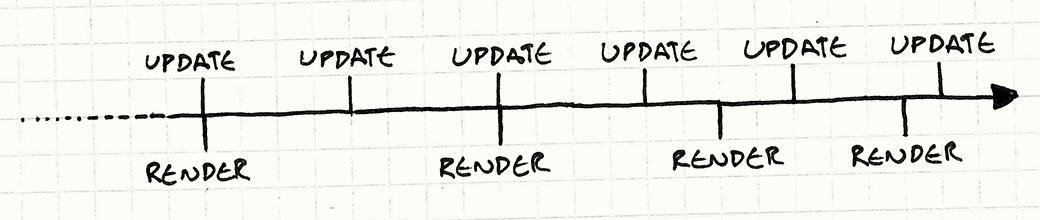
\includegraphics[width=\textwidth]{game-loop-timeline}
    \begin{itemize}
        \pause\item Rendering at ``irregular'' intervals (with respect to update) can result in
            jerky movement 
        \pause\item Solution: \textbf{interpolate} between the two previous updates
            \begin{itemize}
                \pause\item E.g.\ if the render falls exactly halfway between two updates,
                    render each object exactly halfway between its positions
                    \textbf{before} and \textbf{after} the most recent update
            \end{itemize}
    \end{itemize}
\end{frame}

\begin{frame}{Further information on fixed time steps}
    \begin{itemize}
        \item \url{http://gafferongames.com/game-physics/fix-your-timestep/}
        \item \url{http://gameprogrammingpatterns.com/game-loop.html}
    \end{itemize}
\end{frame}

\begin{frame}{Substepping}
    \begin{itemize}
        \pause\item Aims to be a ``best of both worlds'' between fixed and variable time steps 
        \pause\item Use fixed time step at low frame rates, variable at high frame rates 
        \pause\item E.g.\ again with a target update rate of 50Hz 
        \pause\item If refresh rate $<$ 50Hz, update several times per frame, with a \lstinline{deltaTime} of $\frac{1}{50}$ 
        \pause\item If refresh rate $>$ 50Hz, update once every frame, with \lstinline{deltaTime} measured as for variable time step
    \end{itemize}
\end{frame}

\begin{frame}[fragile]{Substepping}
    \begin{lstlisting}[basicstyle=\tiny\ttfamily]
bool running = true;
float lastFrameTime = getCurrentTime();
float timePerUpdate = 1.0f / 50.0f;

while (running)
{
  float currentFrameTime = getCurrentTime();
  float deltaTime = currentFrameTime - lastFrameTime;

  if (deltaTime <= timePerUpdate)
  { // Variable time step
    update(deltaTime);
  }
  else
  { // Fixed time step
    while (deltaTime > 0)
    {
      update(timePerUpdate);
      deltaTime -= timePerUpdate;
    }
  }
  
  render();
  waitForVerticalRefresh();
  lastFrameTime = currentFrameTime;
}
    \end{lstlisting}
\end{frame}

\begin{frame}{Time steps in Unreal}
    \begin{itemize}
        \pause\item Unreal uses \textbf{variable time step} by default
        \pause\item Can be switched to use \textbf{substepping}
        \pause\item \lstinline{Tick} function on C++ classes is called once per frame
        \pause\item \lstinline{FCalculateCustomPhysics} delegate can be used to do something once per substep
        \pause\item Blueprints are updated once per frame; substep updates require C++
        \pause\item More info: \url{http://www.aclockworkberry.com/unreal-engine-substepping/}
    \end{itemize}
\end{frame}

\begin{frame}{Time steps in Unity}
    \begin{itemize}
        \pause\item Unity uses both \textbf{fixed} and \textbf{variable time step}
        \pause\item \lstinline{Update} function on \lstinline{MonoBehaviour}s is tied to frame rate
        \pause\item \lstinline{FixedUpdate} function is tied to fixed physics updates
    \end{itemize}
\end{frame}
